\documentclass[12pt,a4paper]{article}
\usepackage{ctex}
\usepackage{amsmath,amscd,amsbsy,amssymb,latexsym,url,bm,amsthm}
\usepackage{epsfig,graphicx,subfigure}
\usepackage{enumitem,balance}
\usepackage{wrapfig}
\usepackage{mathrsfs,euscript}
\usepackage[usenames]{xcolor}
\usepackage{hyperref}
\usepackage[vlined,ruled,linesnumbered]{algorithm2e}
\usepackage{array}
\hypersetup{colorlinks=true,linkcolor=black}

\newtheorem{theorem}{Theorem}
\newtheorem{lemma}[theorem]{Lemma}
\newtheorem{proposition}[theorem]{Proposition}
\newtheorem{corollary}[theorem]{Corollary}
\newtheorem{exercise}{Exercise}
\newtheorem*{solution}{Solution}
\newtheorem{definition}{Definition}
\theoremstyle{definition}

\renewcommand{\thefootnote}{\fnsymbol{footnote}}

\newcommand{\postscript}[2]
 {\setlength{\epsfxsize}{#2\hsize}
  \centerline{\epsfbox{#1}}}

\renewcommand{\baselinestretch}{1.0}

\setlength{\oddsidemargin}{-0.365in}
\setlength{\evensidemargin}{-0.365in}
\setlength{\topmargin}{-0.3in}
\setlength{\headheight}{0in}
\setlength{\headsep}{0in}
\setlength{\textheight}{10.1in}
\setlength{\textwidth}{7in}
\makeatletter \renewenvironment{proof}[1][Proof] {\par\pushQED{\qed}\normalfont\topsep6\p@\@plus6\p@\relax\trivlist\item[\hskip\labelsep\bfseries#1\@addpunct{.}]\ignorespaces}{\popQED\endtrivlist\@endpefalse} \makeatother
\makeatletter
\renewenvironment{solution}[1][Solution] {\par\pushQED{\qed}\normalfont\topsep6\p@\@plus6\p@\relax\trivlist\item[\hskip\labelsep\bfseries#1\@addpunct{.}]\ignorespaces}{\popQED\endtrivlist\@endpefalse} \makeatother

\begin{document}
\noindent

%========================================================================
\noindent\framebox[\linewidth]{\shortstack[c]{
\Large{\textbf{Lab07-Amortized Analysis}}\vspace{1mm}\\
CS214-Algorithm and Complexity, Xiaofeng Gao, Spring 2020.}}
\begin{center}
\footnotesize{\color{red}$*$ If there is any problem, please contact TA Shuodian Yu. }

\footnotesize{\color{blue}$*$ Name: Futao Wei  \quad Student ID: 518021910750 \quad Email: weifutao@sjtu.edu.cn}
\end{center}
\begin{enumerate}
	\item For the TABLE-DELETE Operation in Dynamic Tables, suppose we construct a table by multiplying its size by $\frac 23$ when the load factor drops below $\frac 13$. Using \emph{Potential Method} to prove that the amortized cost of a TABLE-DELETE that uses this strategy is bounded above by a constant.
	\begin{solution}
		We start by defining a potential function
		\[\Phi (T) = size[T] - num(T)\]
		\textbf{Correctness:} the potential is $0$ for an empty table, and $\Phi (T)$ never goes negative. Thus, the total amortized cost of a sequence of $n$ TABLE-DELETE operations with respect to $\Phi$ is an upper bound of the actual cost. \\
		\textbf{Case 1:} no contraction 
		\begin{align*}
			\hat{C_i} & = C_i + \Phi_i - \Phi_{i-1} \\
			& = 1 + (size_i - num_i) - (size_{i-1} - num_{i-1}) \\
			& = 2
		\end{align*}
		\textbf{Case 2:} a contraction is triggered
		\begin{align*}
			\hat{C_i} & = C_i + \Phi_i - \Phi_{i-1} \\
			& = num_i + 1 + (size_i - num_i) - (size_{i-1} - num_{i-1}) \\
			& = num_{i-1} + 1 - \frac{1}{3} size_{i-1} \\
			& = 1
		\end{align*}
		Hence the amortized cost of a TABLE-DELETE that uses this strategy is bounded above by a constant.
	\end{solution}
	
	\item A \textbf{multistack} consists of an infinite series of stacks $S_0, S_1, S_2,\cdots$, where the $i^{th}$ stack $S_i$ can hold up to $3^i$ elements. Whenever a user attempts to push an element onto any full stack $S_i$, we first pop all the elements off $S_i$ and push them onto stack $S_{i+1}$ to make room. (Thus, if $S_{i+1}$ is already full, we first recursively move all its members to $S_{i+2}$ .) An illustrative example is shown in Figure \ref{Fig-MultiStack}. Moving a single element from one stack to the next takes $O(1)$ time. If we push a new element, \underline{we always intend to push it in stack $S_0$}.

	\begin{figure}[!htbp]
	\centering
	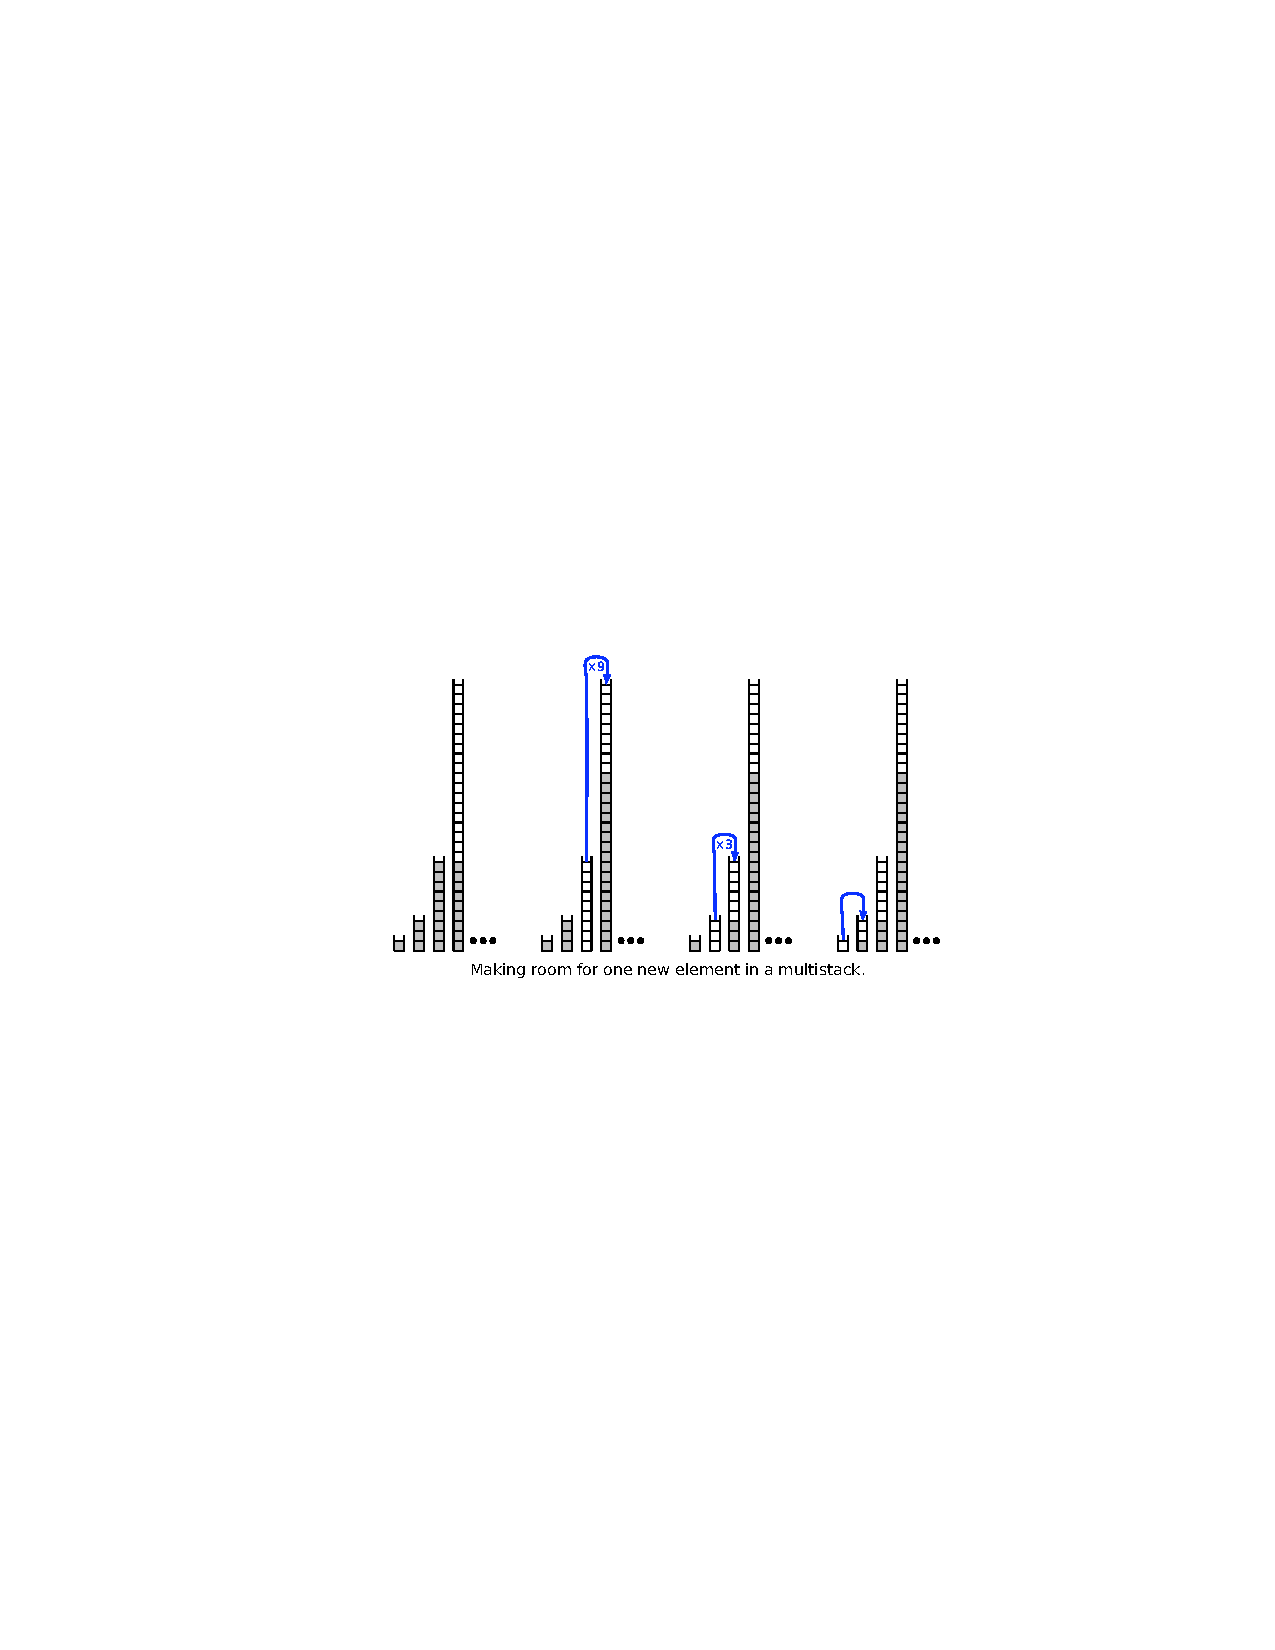
\includegraphics[width=0.5\textwidth]{Fig-MultiStack.pdf}
	\caption{An example of making room for one new element in a multistack.}
	\label{Fig-MultiStack}
	\end{figure}

    \begin{enumerate}
        \item In the worst case, how long does it take to push a new element onto a multistack containing $n$ elements?
        \item Prove that the amortized cost of a push operation is $O(\log n)$ by \emph{Aggregation Analysis}.
        \item {\color{red}(Optional Subquestion with Bonus)} Prove that the amortized cost of a push operation is $O(\log n)$ by \emph{Potential Method}.
    \end{enumerate}
	\begin{solution}
		\hfill
		\begin{enumerate}
			\item 
			In the worst case, $n = \sum\limits_{i=0}^k 3^i$, where pushing a new element requires $n$ pops and $n$ pushes first. Hence $T(n) = 2n + 1$.
			\item
			$S_i$ becomes full every $3^i$ pushes since the first time $S_0, S_1, \cdots , S_{i-1}$ becomes full. Hence the total cost for $S_i$ is
			\[\frac{n - \frac{3^i-1}{2}}{3^i} \cdot 2 \cdot 3^i \sim n , \quad i = 0,1, \cdots\]
			Since there are approximately $\log n$ stacks, we have the aggregate cost $\sim n \log n$. Thus the amortized cost of a push operation is $O(\log n)$.
			\item
			We start by defining a potential function
			\[\Phi (T) = \sum_{i=0}^{k} num_i \cdot (k-i)\]
			where $num_i$ stands for the number of elements in $S_i$ and $k$ for the number of non-empty stacks. \\
			Suppose that the elements in $S_0, S_1, \cdots , S_j (j \geq 0)$ are shifted right after pushing a new element, we have
			\[C_i \leq \sum_{t=0}^{j} 3^t = \frac{3^{j+1} - 1}{2}\]
			Hence the amortized cost of a push operation is
			\begin{align*}
				\hat{C_i} & = C_i + \Phi_i - \Phi_{i-1} \\
				& \leq  \frac{3^{j+1} - 1}{2} + \sum_{t=1}^{j} 3^{t-1} \cdot (k-t) + 3^j \cdot (k-j-1) - \sum_{t=0}^{j} 3^{t} \cdot (k-t) \\
				& \sim k \\
				& \sim O(\log n)
			\end{align*}
			
		\end{enumerate}
	\end{solution}
	
	\item Given a graph $G = (V, E)$, and let $V'$ be a strict subset of $V$. Prove the following propositions.
	
	\begin{enumerate}
		\item Let $T$ be a minimum spanning tree of a $G$. Let $T'$ be the subgraph of $T$ induced by $V'$, and let $G'$ be the subgraph of $G$ induced by $V'$. Then $T'$ is a minimum spanning tree of $G'$ if $T'$ is connected.
		\item Let $e$ be a minimum weight edge which connects $V'$ and $V \setminus V'$. There exists a minimum weight spanning tree which contains e.
	\end{enumerate}
	\begin{solution}
		\hfill
		\begin{enumerate}
			\item 
			If $T'$ is connected, then $T'$ is obviously a tree. \\ Suppose for contradiction that $T'$ is not a minimum spanning tree of $G'$ and $S$ is one. In this case, we can get a spanning tree of $G$ by connecting $S$ with $T \setminus T'$, which is smaller than $T$ --- we get a contradiction! Hence $T'$ is a minimum spanning tree of $G'$. 
			\item
			Assume for contradiction that no minimum weight spanning tree contains $e$. But any minimum spanning tree has to connect $V'$ and $V \setminus V'$ via a certain edge, say, $e'$. If we replace $e'$ with $e$, we'll get a spanning tree which is no worse than minimum, since $e$ is a minimum weight edge which connects $V'$ and $V \setminus V'$. --- A contradiction! The proposition is thus proved.
		\end{enumerate}
	\end{solution}
\end{enumerate}



\textbf{Remark:} Please include your .pdf, .tex files for uploading with standard file names.


%========================================================================
\end{document}
